\chapter{Theoretische Grundlagen}
\label{chap:theoretische_grundlagen} Dieses Kapitel führt in die theoretischen Grundlagen
ein, die in dieser Arbeit benötigt werden. Den ersten Teil bilden die domänenspezifischen
Grundlagen \ref{sec:domänenspezifisch}, welche genauer darauf eingehen, welchen Inhalt
die zu bearbeitenden Bilder bieten und wie diese zu verstehen sind. Abschnitt
\ref{sec:technologisch} geht anschließend genauer auf die Bildgebung ein, die eine
wichtige Rolle spielen. Der Abschnitt \ref{sec:verwwandte_arbeit} geht auf die
Arbeit von Herrn Hofmann ein, welche das zugrundeliegende Verfahren beschreibt.
Der Abschnitt \ref{sec:3d_slicer} führt in Softwareentwicklungsthemen ein, die zum
Erstellen einer 3D Slicer Erweiterung wichtig sind.
% ---------------------------------------------------------------------------------------

\section{Domänenspezifisch}
\label{sec:domänenspezifisch} Wie bereits aus dem Kapitel \ref{chap:einleitung} Einleitung
klar wurde, handelt es sich bei den Mikro-\ac{CT}-Bildern um Zahnbilder. Um zu
verstehen, wie eine \ac{CT}-Aufnahme technisch segmentiert und damit zerlegt
werden kann, muss zunächst die Zahnstruktur selbst verstanden werden.

\begin{minipage}{0.40\textwidth}
	Die Abbildung \ref{fig:aufbau_eines_zahnes} zeigt den groben Aufbau eines Zahnes
	nach \citet[S.~17]{lehmann2012Zahnheilkunde}. Zu sehen ist, dass das Denit
	oder auch Zahnbein genannt den Großteil eines Zahnes einnimmt. Im Bereich der Zahnkrone
	wird das Dentin von Zahnschmelz überzogen. Der Zahnschmelz ragt in die
	Mundhöhle und ist nach \citet[S.~41]{lehmann2012Zahnheilkunde} das härteste Material
	im menschlichen Körper. In der Mitte des Zahnes befindet sich Weichgewebe, das
	als Pulpa bezeichnet wird vgl. \citep[vgl.][S.~15]{lehmann2012Zahnheilkunde}.
\end{minipage}
\hfill
\begin{minipage}{0.50\textwidth}
	\centering
	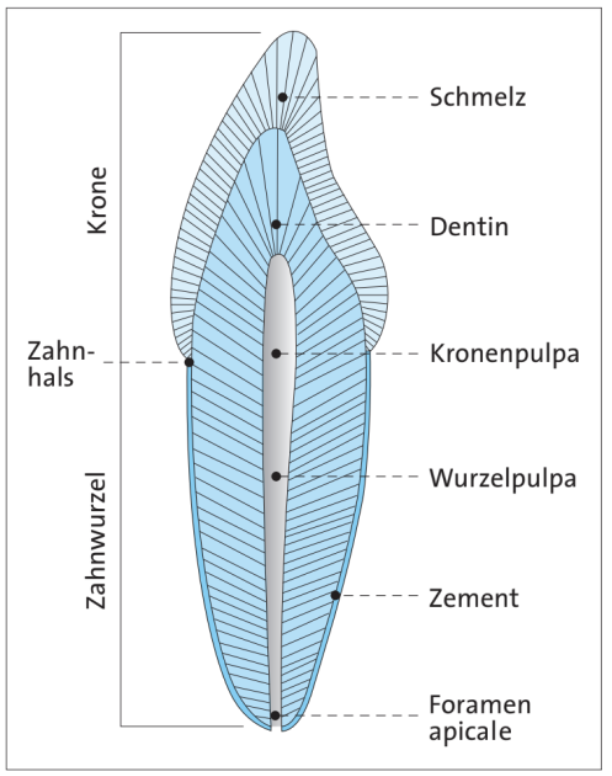
\includegraphics[scale=0.50]{img/aufbau_eines_zahns.jpg}
	\captionof{figure}{Aufbau eines Zahnes nach \citet[S.~15]{lehmann2012Zahnheilkunde}}
	\label{fig:aufbau_eines_zahnes}
\end{minipage}

Für die Bearbeitung von Mikro-\ac{CT}-Aufnahmen sind die Bereiche Schmelz,
Dentin und Pulpa von besonderer Bedeutung. Betrachtet man eine \ac{CT} wie es zu
Beginn in der Abbildung \ref{fig:ct_aufnahme_eines_zahns} gezeigt wurde, so bilden
diese drei Gewebearten die unterschiedlichen Grauwerte in einem \ac{CT}-Bild.

\begin{description}
	\item[\textbf{Die Pulpa}] unterscheidet sich hierbei nur wenig vom Hintergrund,
		da sie als einzige der drei Hauptteile eines Zahnes ein Weichgewebe ist und
		bei einer Röntgenaufnahme nicht absorbiert. Dieser Teil ist in dieser Arbeit
		weniger relevant und auch nicht Teil des Verfahrens, was das
		Segmentierungsverfahren eher zu einer Zahnkronensegmentierung macht. Geht man
		weiter von innen nach außen, so ist der nächste Zahnteil auf einem \ac{CT} das
		Zahnbein.

	\item[\textbf{Das Dentin}] ist laut \citet[S.~41]{lehmann2012Zahnheilkunde}
		eine Hartsubstanz, die dem Kieferknochen sehr nah steht. So kommt es, dass dieser
		Teil schon deutlich besser auf einem \ac{CT} zu erkennen ist. Den äußersten Teil
		in der Mundhöhle bildet das Zahnschmelz.

	\item[\textbf{Der Schmelz}] ist der härteste Teil im menschlichen Körper und aus
		diesem Grund auch am hellsten auf dem \ac{CT} zu erkennen.
\end{description}

Die folgende Abbildung \ref{fig:pulpa_dentin_schmelz} soll die unterschiedlichen
Graubereiche den einzelnen Zahnsubstanzen auf einer \ac{CT}-Aufnahme zuordnen.

\begin{figure}[h]
	\centering
	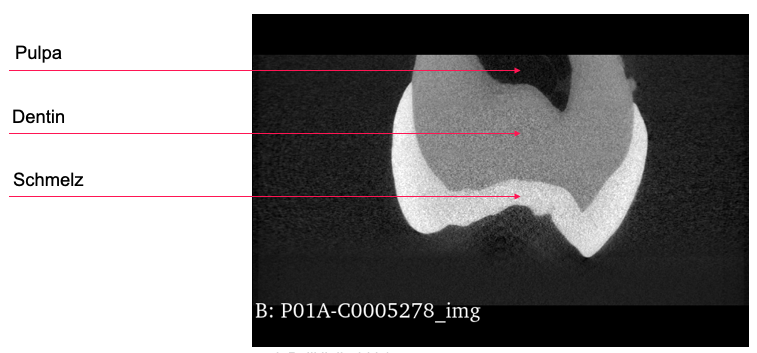
\includegraphics[width=0.9\textwidth]{img/dentin_schmelz_pulpa.png}
	\caption{Darstellung von Pulpa, Dentin und Schmelz auf einer CT-Aufnahme nach \citet{heck2024}}
	\label{fig:pulpa_dentin_schmelz}
\end{figure}

Mit diesem Domänenwissen kann ein Schritt weiter gegangen werden, sodass der
Fokus nun auf die \ac{CT}-Bilder gesetzt wird. Das Kapitel
\ref{sec:technologisch} Bildgebung führt die Technologie der Computertomografie
tiefer ein. Darüber hinaus werden die verschiedenen Formate und statistische Modelle
der \ac{CT}-Aufnahmen vorgestellt.
% ---------------------------------------------------------------------------------------

\section{Bildgebung}
\label{sec:technologisch} Es gibt die unterschiedlichsten Arten zur Erzeugung
dreidimensionaler Bilddaten. Dieser Abschnitt erläutert federführend die Technologie
der Mikro-\ac{CT}-Aufnahmen und deren Erstellung. Diese sind für einen medizinischen
Einsatz besonders interessant. Des Weiteren erfolgt eine Einführung in die
Speicherung und Komprimierung von \ac{CT}-Aufnahmen. Das sorgt dafür, dass die digitalen
Bilddaten deutlich handlicher werden.
% ---------------------------------------------------------------------------------------

\subsection{Computertomografie}
\label{subsec:computertomografie} Die Erfindung der Computertomografie (\ac{CT})
war ein Quantensprung in der Geschichte der Medizin. Sie ist aus heutigen Diagnosen
nicht mehr wegzudenken. Ein Mikro-\ac{CT}-Bild ist laut \citet[S.~1]{baird2017}
ein Menge hochauflösender Bilder, die wie ein Stapel zusammengelegt werden. Der
Aspekt Mikro deutet dabei darauf hin, dass es eine miniaturisierte Ausführung eines
üblichen Kegelstrahl-\ac{CT}s ist, so \citet[S.~340]{buzug2011}. Eine andere
Definition erläutert \citet[S.~49]{lehmann2013bildverarbeitung}. Er beschreibt
die Computertomografie als Projektionen einzelner Ebenen im Untersuchungsobjekt.
Die Technologie, mit der diese Bilderstapel aufgenommen werden, ist unter der Röntgentechnik
oder auch \ac{X-Ray} bekannt. Die Röntgenstrahlung ist eine Form der elektromagnetischen
Strahlung, ähnlich wie das sichtbare Licht, so das \citet[K.~1]{nib2024}. Anders
als das Licht haben die Röntgenstrahlen eine viel höhere Energie. Das führt dazu,
dass man mit dieser elektromagnetischen Strahlung viele Objekte durchdringt werden
können. So auch Gewebeteile eines Zahnes \citep[vgl.][K.~1]{nib2024}. Die
Abbildung \ref{fig:spectrum} zeigt dieses elektromagnetische Spektrum.

\begin{figure}[h]
	\centering
	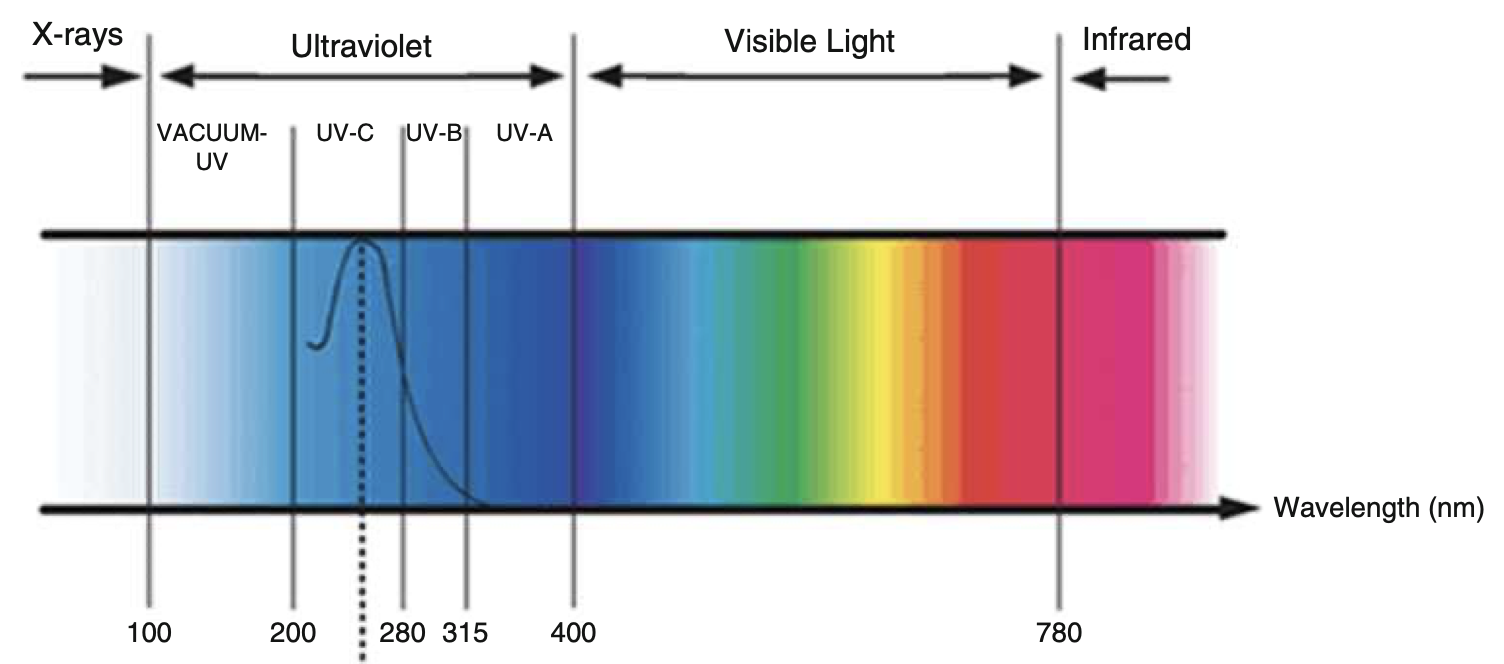
\includegraphics[width=0.6\textwidth]{img/x_ray.jpg}
	\caption{Einordnung von X-Ray nach \citet[S.~5]{zwinkels2015}}
	\label{fig:spectrum}
\end{figure}

Durchdringt ein solcher Röntgenstrahl ein Untersuchungsobjekt, werden die
Details aufgrund der Wechselwirkung mit Materie auf einer \ac{CT}-Probe sichtbar.
Die bekannteste Wechselwirkung ist die Absorption. Mit der Steigerung der Atomzahl
in einem Material nimmt auch die Absorption eines Materials zu, sodass es leicht
ist verschiedene Materialien in einer \ac{CT}-Aufnahme zu unterscheiden \citep[vgl.][K.~1]{nib2024}.

Für eine Mikro-\ac{CT}-Aufnahme bedarf es spezieller Technik. Es gibt
unterschiedliche Firmen, welche die unterschiedlichsten Modelle anbieten. Im
Falle der Zahnklinik an der \ac{LMU} handelt es sich um ein Mikro-\ac{CT}-Gerät
der Firma \citet{scanco2024}. Dieses Gerät erstellt Aufnahmen mittels
Röntgenstrahlung und generiert mithilfe der Computertomografie ein
dreidimensionales Bild, welches im Format \ac{ISQ} abgelegt wird. Wie das nächste
Kapitel beschreiben wird, ist der Speicherumfang den solch ein Bild benötigt
sehr groß, jedoch auch sehr detailliert. Um ein einfacheres Arbeiten mit den \ac{CT}-Bildern
zu ermöglichen, kann eine simple Technik angewendet werden, die hier beschrieben
werden soll.
% ---------------------------------------------------------------------------------------

\subsection{Datenformate}
\label{subsec:datensätze} Die rohen Datensätze, welche direkt aus dem Mikro-\ac{CT}-Gerät
kommen, haben nach \citet{scanco2024} das Format \ac{ISQ}. Dieses Format fällt speziell
auf die Geräte der Firma SCANCO zurück. Wie das vorherige Kapitel
\ref{subsec:computertomografie} bereits eingeführt hat, ist dieser Dateityp für eine
weitere Bearbeitung nur bedingt geeignet. Unter anderem wegen ihrer Größe. \citet{RoeschKunzelmann2018}
haben hierfür ein Paket entwickelt. Dieses konvertiert ein \ac{ISQ} Format in
ein \ac{mhd} Format. Bei einer \ac{mhd} Datei handelt es sich um ein Metafile,
dass auf die eigentliche Datei verweist. Folgender Ausschnitt zeigt die Verwendung
des Pakets.
\begin{center}
	\texttt{python3 isq\_to\_mhd.py <quelle> <ziel>}
\end{center}
Diese Metadatei kann genutzt werden, um interessante Informationen über das Bild
zu erlangen. Wird dieses Kommando ausgeführt, so erstellt das Skript \texttt{isq\_to\_mhd}
ein Metafile, das detaillierte Daten über die Datei enthält. Ein Ausschnitt
dieses Metafiles liefer das Listing \ref{lst:inhalt_mhd_datei}

\begin{lstlisting}[
	caption={Ausschnitt des Inhaltes einer mhd-Datei},
	label={lst:inhalt_mhd_datei}]
ObjectType = Image
NDims = 3
CenterOfRotation = 0 0 0
ElementSpacing = 0.02 0.02 0.02
DimSize = 1024 1024 517
ElementType = MET_SHORT
ElementDataFile = P01A-C0005278.ISQ
\end{lstlisting}

In der Datei sind Informationen über die Ausprägung, Art und Größe der Datei zu finden.
Besonders interessant sind die Punkte \texttt{DimSize und ElementType}. Über
diese Parameter lässt sich die Größe eines Bildes berechnen. \citet[S.~10-11]{burger2009}
erklärt, dass ein Bild in Zellen aufgeteilt ist, welche Informationen enthalten.
Diese Zellen sind im zweidimensionalen Raum als Pixel bekannt. Betrachtet man
jedoch ein, wie im Falle der Zahnklinik an der \ac{LMU} dreidimensionales Bild, so
spricht man nicht mehr von einem Pixel, sondern von einem Voxel. Ein Voxel ist demnach
das dreidimensionale Äquivalent zu einem Pixel. \citet[S.~10-11]{burger2009} beschreiben
weiter das jeder diese Zellen ein binäres Wort der Länge $2^{k}$ ist. Die Basis
2 ergibt sich durch das binäre Wort, wo hingegen für $k$ gilt:
$k \in \mathbb{N}$. Um für den konkreten Fall aus Listing \ref{lst:inhalt_mhd_datei}
das entsprechenden $k$ zu ermitteln, muss der \texttt{ElementType} näher betrachtet
werden. \texttt{MET\_SHORT} steht hierbei für Signed short, was eine Größe von
16 Bit entspricht. Damit ergibt sich für die Länge $k$ ein Wert von 4. So können
nach \citet[S.~10-11]{burger2009} folgende Gleichungen festgehalten werden.

\begin{align}
	\label{equ:größe_bestimmen}1024 \cdot 1024 \cdot 517    & = 542,113,792 \, \text{Voxel}\notag  \\
	542,113,792 \, \text{Voxel}\cdot 2 \, \text{Byte/Voxel} & = 1,084,227,584 \, \text{Byte}\notag \\
	1,084,227,584 / 1,000,000,000                           & = 1.0842 \, \text{GB}
\end{align}

Die erste Gleichung bestimmt die Gesamtzahl aller Voxel in einem Bild. Gleichung
zwei ermittelt die Größe des Bildes in der Einheit Byte. Die letzte Zeile nimmt eine
Umrechnung von Byte nach \ac{GB} vor.

Durch die Gleichungen in \ref{equ:größe_bestimmen} wird klar, dass eine \ac{CT}-Aufnahme
des Typs \ac{ISQ} direkt nach seiner Aufnahme über einen \ac{GB} groß ist. Es stellt
sich also die spannende Frage, wie solch eine Datei komprimiert werden kann, ohne
das es Verluste in der Qualität gibt. Dr. Elisa Walter hat hierfür eine Lösung entwickelt.
Betrachtet man den \texttt{ElementType} genauer, so fällt auf, dass es noch weitere
Typen gibt, die durch eine geringere Länge $k$ deutlich weniger Speicher
benötigen. Durch Anwendung simpler Statistik lässt sich herauslesen, dass die
$2^{4}$ Byte je Element nicht ausgenutzt werden. Als Werkzeug für die Betrachtung
einer solchen Statistik kann das Histogramm eines Bildes genutzt werden. Laut
\citet[S.~249]{jahne2024} ist ein Histogramm die Häufigkeitsverteilung der Grauwerte.
Diese zeigt grafisch die unterschiedlichen Grauwerte (x-Achse) zu ihren
Häufigkeiten im Bild (y-Achse). \citet[S.~249]{jahne2024} macht deutlich, dass das
Histogramm jedoch kein Aufschluss über die räumliche Verteilung der Pixel oder Voxel
liefert. Werden einige der Argumente nicht verwenden, so kann der \texttt{ElementTyp}
verkleinert werden.
% ---------------------------------------------------------------------------------------

\section{Bildbearbeitung}
\label{sec:bildbearbeitung} Nachdem ein \ac{CT} erzeugt und gegebenenfalls komprimiert
wurde, folgt die Bearbeitung eines Bildes. Hierfür bietet das Pipeline-Modell von
\citet[S.~50]{handels2000} eine gute Richtlinie. Er beschreibt mit dieser Visualisierungs-Pipeline
Schritte, die bei der Bearbeitung von dreidimensionalen \ac{CT}-Aufnahmen notwendig
sind \citep[vgl.][S.~50]{handels2000}. Die ersten Schritte, \textit{Bildvorverarbeitung}
und \textit{Segmentierung}, sind von besonderem Interesse. Dieser Abschnitt
orientiert sich an dieser Unterteilung und nimmt sie sich als Vorbild. Daraus ergeben
sich die Abschnitte \ref{subsec:filter} Filter und \ref{subsec:segmentierung} Segmentierung,
welche die Pipelineschritte \textit{Bildvorverarbeitung} und \textit{Segmentierung}
wiederspiegeln sollen.
% ---------------------------------------------------------------------------------------

\subsection{Filter}
\label{subsec:filter} \ac{CT}-Aufnahmen rauschen, dies ist ein Fakt und liegt in
der Natur einer Röntgenaufnahme. Dies beschreiben auch \citet[K.~3]{diwakar2018}
in ihrem Paper über \ac{CT}-Bildrauschen und Entrauschen. Dabei liegt die
Ursache des Rauschens nicht an einer Stelle, sondern ist auf viele Quellen zurückzuführen.
Eine gute Einteilung dieser Quellen liefern ebenfalls \citet[K.~3]{diwakar2018}.
Sie teilen die Rauschquellen auf in \textit{Random noise, Statistical noise,
Electronic noise} und \textit{roundoff noise}.

Unter dem Rauschen eines Bildes versteht man die Streuung der Pixelwerte im Bild.
Für eine Segmentierung des Bildes ist dieses Verhalten unerwünscht und führt zu schlechten
Ergebnissen \citep[vgl.][S.~51]{handels2000}. Die Bildvorverarbeitung oder auch Filter
genannt, hat die Aufgabe dieses Rauschen so gut wie möglich zu reduzieren. Hierzu
gibt es diverse Möglichkeiten.

\begin{minipage}{0.40\textwidth}
	Mit Blick auf die folgenden Kapitel sind für diese Arbeit vor allem die lokalen
	Operatoren relevant. Die lokalen Operatoren sind charakteristisch für die
	Betrachtung der lokalen Nachbarschaft. Jeder Pixel betrachtet also seine Umgebung
	und führt auf Basis darauf eine Berechnung des jeweils betrachteten Pixels durch.
	In Abbildung \ref{fig:lokaler_operator_maske} ist der aktuellen Pixel der, mit
	der Position $P = (0/0)$ \citep[vgl.][S.~52]{handels2000}.
\end{minipage}
\hfill
\begin{minipage}{0.50\textwidth}
	\centering
	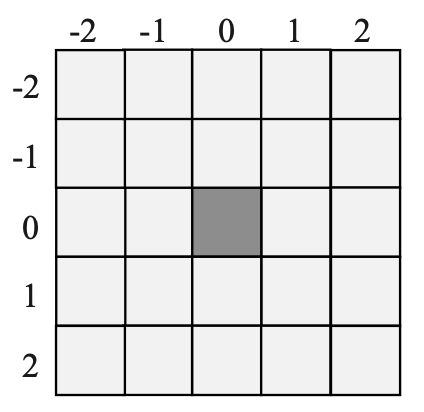
\includegraphics[width=0.60\textwidth]{img/lokaler_operator_maske.jpg}
	\captionof{figure}{Maske eines lokalen Operators nach \citet[S.~52]{handels2000}}
	\label{fig:lokaler_operator_maske}
\end{minipage}

Für die konkrete Betrachtung der Nachbarschaft eines Pixels empfiehlt \citet[S.~52]{handels2000}
eine Maske (Ausschnitt) heranzuziehen, die mit einer Matrix interpretiert werden
kann und die Nachbarschaft eines Pixels abbildet. Abbildung \ref{fig:lokaler_operator_maske}
zeigt eine solche Maske und soll das Verfahren so verdeutlichen. Der grau
hinterlegte Mittelpunkt - $P = (0/0)$ - ist das aktuell betrachtete Pixel. Die Felder
um die Mitte herum die Nachbarn. Es fällt jedoch auf, dass durch dieses Schema nicht
jede mögliche Ausprägung einer Maske infrage kommt. Um einen Mittelpunkt und
damit ein aktuelles Pixel betrachten zu können, bedarf es eines ungeraden Grades
für $M$. Diese Eingrenzung lässt sich in Gleichung \ref{equ:lokaler_operator}
generisch fassen.

\begin{align}
	\label{equ:lokaler_operator}M_{(2_m+1)x(2_m+1)} & = \begin{bmatrix}k_{11}&k_{12}&k_{13}\\ k_{21}&x&k_{23}\\ k_{31}&k_{32}&k_{33}\\\end{bmatrix} & m \in \mathbb{N}
\end{align}

Die Gleichung \ref{equ:lokaler_operator} beschreibt die mögliche Ausprägung eines
lokalen Operators als Matrix. Dabei sei $m \in \mathbb{N}$. Die Variable $x$ beschreibt
das aktuell betrachtete Pixel, während $k_{nn}$ die Nachbarn illustrieren soll. Durch
die Gleichung ist auch zu erkennen, dass die Maske des lokalen Operators
beliebig groß werden kann. Eine hohe Ordnung der Operatormatrix ist jedoch nicht
immer von Vorteil, sodass es letzten Endes auf den Anwendungsfall ankommt.

Mit der Technik der lokalen Operatoren können nun unterschiedliche Arten
angewendet werden. \citet[S.~54 - 55]{handels2000} unterscheidet hier in
Glättungsfilter, Mittelwertfilter, Medianfilter, Gaußfilter und Binomialfilter.
Alle dieser Filter bedienen sich einer Operatormaske, um auf Basis der Nachbarelemente
einen statistischen Wert für den Bildpunkt zu erhalten. Um einen genaueren
Einblick in alle Filter zu erlangen, sei an dieser Stelle auf \citet[S.~54 - 55]{handels2000}
verwiesen.

Wie zu Anfang dieses Kapitels beschrieben, ist eine Bildvorverarbeitung (Filterung)
für eine gute Segmentierung des Bildes unerlässlich. So kommt es das auch in der
Visualisierungs-Pipeline nach \citet[S.~50]{handels2000} der zweite Schritt bereits
die Segmentierung einführt. Warum dies so ein wichtiger Bestandteil der
Bildanalyse ist und welche Methoden sich hier bieten, erläutert das folgende Kapitel.
% ---------------------------------------------------------------------------------------

\pagebreak

\subsection{Segmentierung}
\label{subsec:segmentierung} Die Bildsegmentierung oder auch Bildaufteilung
genannt, ist ein wichtiges Teilgebiet der Bildverarbeitung und beschäftigt sich mit
der Bildanalyse. Ihr Ziel ist es, detaillierte beschreibende Bilder aus dem vorliegenden
Originalbild zu berechnen. Dies kann im Falle eines \ac{CT}s der Zahnklinik an
der \ac{LMU} die hervorgehobene Darstellung der Zahnsubstanzen Schmelz und Dentin
sein. \citep[vgl.][S.~359]{lehmann2013bildverarbeitung}. Konkret teilt ein
Segmentierungsverfahren also ein Bild in Teilbereiche auf. Dabei sind die Teilbereiche
in sich bemerkenswert homogen. \citet[S.~1]{ramesh2021} beschreiben, dass der
Prozess der Segmentierung zur Gewinnung wichtiger Informationen dient wie zum
Beispiel die Zahnkaries Ausbreitung. So kommt es, dass \citet[S.~50]{handels2000}
in seiner Visualisierungs-Pipeline die Segmentierung als zweiten Schritt und damit
als zentrales Problem darstellt. \citet[S.~95]{handels2000} und \citet[S.~360]{lehmann2013bildverarbeitung}
beschreiben beide, dass die Bildsegmentierung eines \ac{CT}s für eine gute und eindeutige
ärztliche Diagnose nicht mehr wegzudenken ist. Warum dem so ist, verdeutlicht die
Abbildung \ref{fig:interpretation_einer_ct_aufnahem}.

\begin{figure}[h]
	\centering
	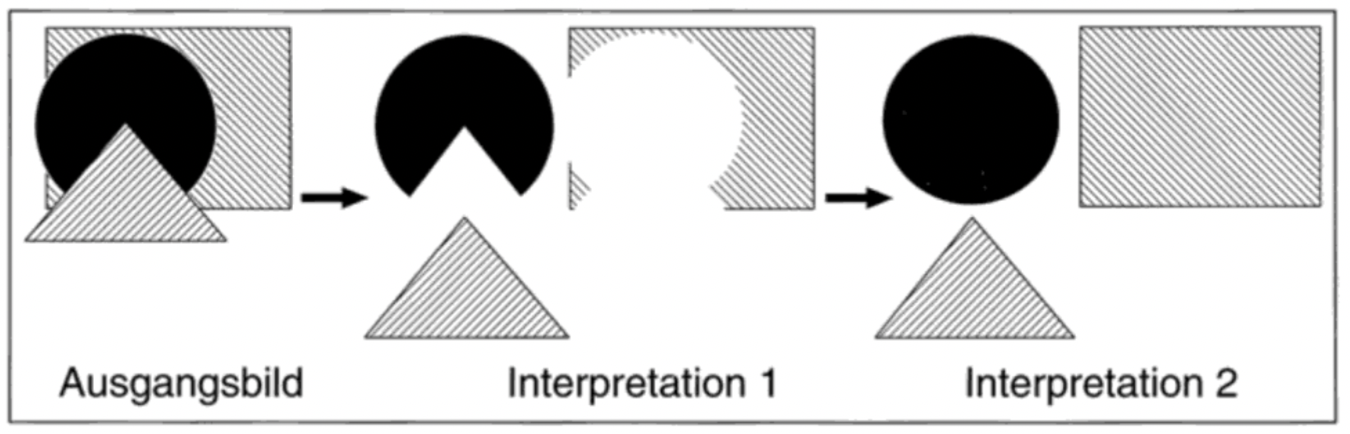
\includegraphics[width=0.8\textwidth]{img/bild_interpretation.jpg}
	\caption{Interpretation einer CT-Aufnahme nach \citet[S.~360]{lehmann2013bildverarbeitung}}
	\label{fig:interpretation_einer_ct_aufnahem}
\end{figure}

Zu erkennen ist das originale Bild (Ausgangslage) und mögliche
Interpretationsschritte (Interpretation 1 und Interpretation 2). \citet[S.~360]{lehmann2013bildverarbeitung}
verdeutlichen mit dieser Abbildung \ref{fig:interpretation_einer_ct_aufnahem}, dass
mittels Segmentierung die einzig mögliche Interpretation die Erste ist. Auch
wenn die zweite Interpretation die deutlich logischere ist, kann diese ohne weitere
Forschung nicht bewiesen werden, so \citet[S.~360]{lehmann2013bildverarbeitung}.
Außerdem ist zu erkennen, dass die Abbildung \ref{fig:interpretation_einer_ct_aufnahem}
die Definition einer Segmentierung belegt. Die Erzeugung inhaltlich
zusammengehöriger Regionen werden hier durch die verschiedenen Formen
visualisiert \citep[vgl.][S.~360]{lehmann2013bildverarbeitung}.

Um ein Bild zu segmentieren, gibt es unzählige Möglichkeiten. Für die Auswahl eines
Verfahrens spielt unter anderem der Anwendungsbereich eine wichtige Rolle. Die
Verfahren, die in dieser Arbeit von Wichtigkeit sind, sind die
Schwellwertverfahren \citep[vgl.][S.~361]{lehmann2013bildverarbeitung}.

\pagebreak

\textbf{Schwellwertverfahren} (engl.: thresholding) gehören zu den Standardwerkzeugen
einer Segmentierung, sodass diese die Basis vieler weiterer Verfahren legen. Bei
einer schwellwertbasierten Segmentierung werden die Pixel eines Bildes anhand von
Schwellwerten eingruppiert \citep[vgl.][S.~96]{handels2000}. Die nachfolgende Gleichung
\ref{equ:schwellwertverfahren} soll dies verdeutlichen.

\begin{align}
	\label{equ:schwellwertverfahren}B(x, y, z) = \begin{cases}1,&\text{falls }t_{\text{unten}}\leq f(x, y, z) \leq t_{\text{oben}}, \\ 0,&\text{sonst}.\end{cases}
\end{align}

$B(x, y, z)$ beschreibt ein Pixel in einem dreidimensionalen Bild, demnach ein Voxel.
Liegen die Werte eines Voxels, also $f(x, y, z)$, innerhalb der beiden
Schwellwerte $t_{oben}$ und $t_{unten}$, dann wird eine 1 zugewiesen. Liegt der
aktuell betrachtete Voxel nicht zwischen den Schwellwerten, so wird eine 0 zugewiesen.
Das Ergebnis einer solchen primitiven Schwellwertsegmentierung ist ein binäres
Bild, welches in Abbildung \ref{fig:binäres_schwellwertverfahren} zu sehen ist.

\begin{figure}[h]
	\centering
	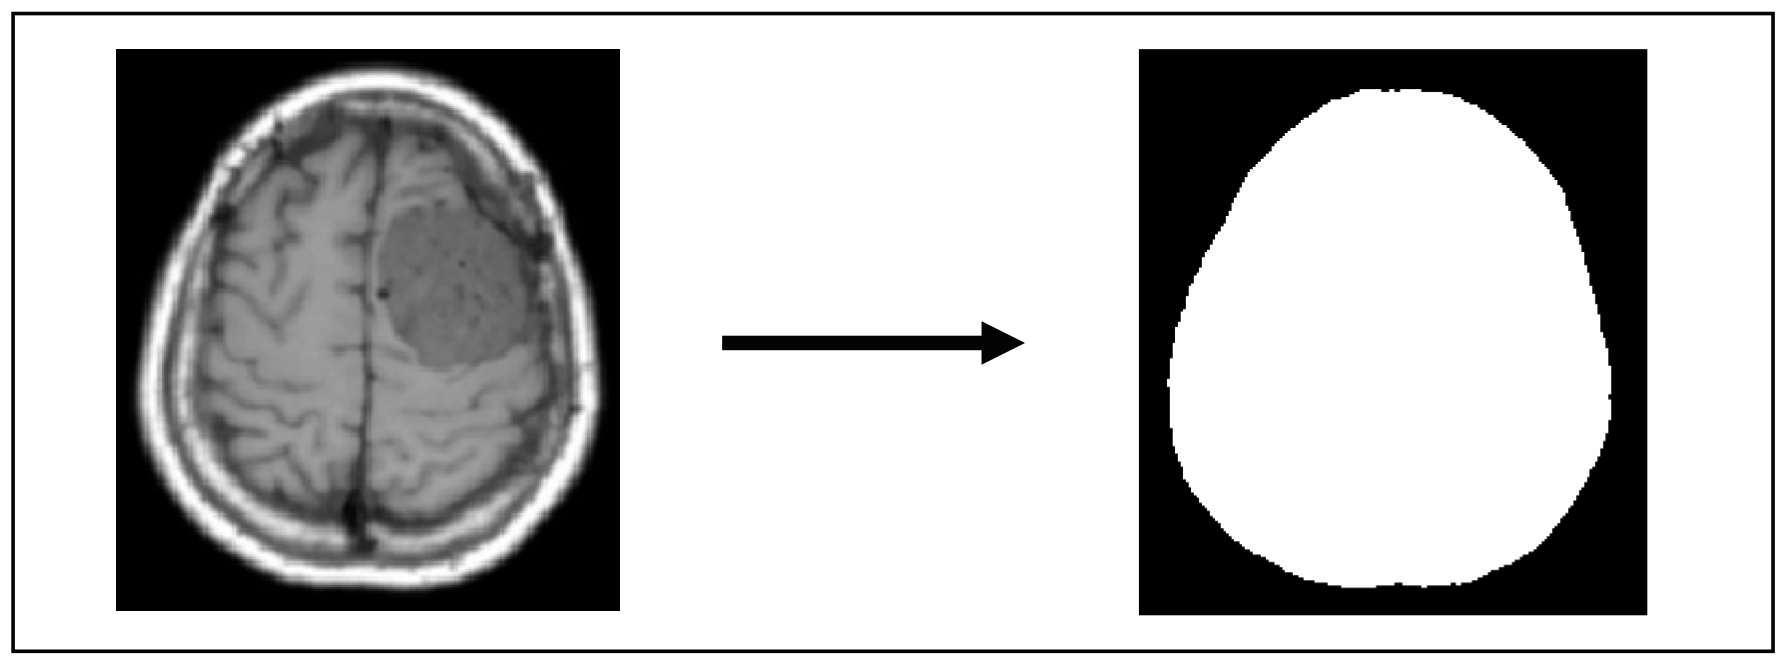
\includegraphics[width=0.8\textwidth]{img/beispiel_schwellwertverfahren.jpg}
	\caption{Ergebnis eines einfachen Schwellwertverfahrens nach \citet[S.~96]{handels2000}}
	\label{fig:binäres_schwellwertverfahren}
\end{figure}

Zu erkennen ist, dass nach einem einfachen Schwellwertverfahren das Bild nur noch
aus zwei unterschiedlichen Graustufen besteht. Betrachtet man das Ergebnis in
\ref{fig:binäres_schwellwertverfahren} genauer, so ist diese einfache Segmentierung
durchaus erfolgreich verlaufen. Der Grund dafür ist die gute Wahl des
Schwellwerts.

Die interessanteste Frage bei den Schwellwertverfahren ist die Wahl des
Schwellwerts $t$. Dieser entscheidet zwischen einer guten und einer schlechten Segmentierung.
Für die Wahl eines Schwellwerts empfiehlt sich der Blick auf das Bildhistogramm.
Dieses gibt Aufschluss über die Verteilung der Grauwerte in einem Bild \citep[vgl.][S.~361]{lehmann2013bildverarbeitung}.
Verfahren, welche einen guten Schwellwert gewährleistet, ohne dass zu viele Informationen
verloren gehen, sind die Verfahren \textit{Otsu} und \textit{Renyi}.

\pagebreak

\textbf{Das Verfahren nach Otsu} gehört zu den Schwellwertverfahren und bestimmt
den Schwellwert $t$ durch ein statistisches Gütekriterium. Hierzu bedient sich das
Verfahren des Bildhistogramms. Die räumliche Anordnung der Voxel und damit das
tatsächliche Bild, benötigt dieser Algorithmus nicht \citep[vgl.][S.~264]{lehmann2013bildverarbeitung}.

\begin{minipage}{0.40\textwidth}
	Ein solches Histogramm, welches die Grundlage für das Verfahren nach Otsu
	liefert, sei in Abbildung \ref{fig:histogramm} gezeigt. Dies gibt Aufschluss
	über die unterschiedlichen Grauwerte und wie oft sie in einem Bild vorkommen
	\citep[vgl.][S.~264]{lehmann2013bildverarbeitung}. Für eine genauere
	Beschreibung eines Histogramms, sei an dieser Stelle auf \citet[S.~42]{burger2009}
	verwiesen.
\end{minipage}
\hfill
\begin{minipage}{0.50\textwidth}
	\centering
	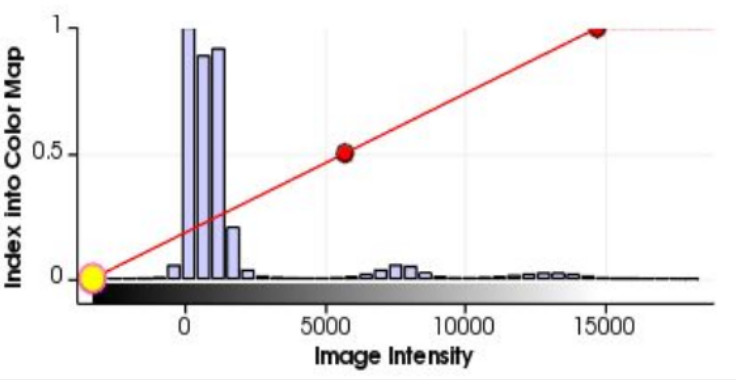
\includegraphics[width=1\textwidth]{img/histogramm.jpg}
	\captionof{figure}{Histogramm einer Zahnaufnahme nach \citet[S.~13]{hoffmann2020}}
	\label{fig:histogramm}
\end{minipage}

Das Otsu-Verfahren teilt die Grauwerte eines Bildes in verschiedenen Klassen ein,
die durch Schwellwerte getrennt werden. Die Klassen können beispielsweise mit $K_{0}$
bis $K_{n}$ bezeichnet werden, wobei sich dieses konkrete Beispiel auf die
Klassen $K_{0}$ und $K_{1}$ beschränkt. Otsu wählt den Schwellwert $t$, der die
Varianz zwischen den Pixelklassen maximiert und gleichzeitig die Varianz
innerhalb jeder Klasse minimiert \citep[vgl.][S.~264]{lehmann2013bildverarbeitung}.
Mathematisch lässt sich dies wie folgt ausdrücken.

\begin{align}
	t = \text{max }(\sigma_{zw}^{2}/ \sigma_{in}^{2})
\end{align}

$\sigma_{zw}$ bildet die Varianz zwischen den beiden Klassen $K_{0}$ und $K_{1}$
und bildet sich aus den Wahrscheinlichkeiten, mit denen jeder einzelne Grauwert
auftritt. $\sigma_{in}$ hingegen, ist die Varianz innerhalb einer Klasse und
entsteht durch die Addition der Varianzen der einzelnen Klassen. Der Schwellwert
$t$ ist nun der, für den das Verhältnis maximal wird \citep[vgl.][S.~264]{lehmann2013bildverarbeitung}.

Laut \citet[S.~264]{lehmann2013bildverarbeitung} fällt auf, dass dieses Verfahren
vorallem bei bimodalen Bildern zum Einsatz kommt. Ein Bild ist bimodal, wenn es zwei
lokale Maxima aufweist. Vereinfacht gesagt, wenn es zwei lokale Piecks enthält \citep[vgl.][S.~264]{lehmann2013bildverarbeitung}.

Eine ähnliche Technik für die Bestimmung des Schwellwerts liefert das Verfahren
der Renyi Entropie. Auch hier ist eine Einteilung der Voxel in Klassen vorgesehen.
% ---------------------------------------------------------------------------------------
\pagebreak

\textbf{Das Verfahren nach Rényi} ist ein weiteres Verfahren, das im Laufe dieser
Arbeit noch eine wichtige Rolle spielt. Wie bereits beschrieben gehört es
ebenfalls zu der Gruppe der Schwellwertverfahren und generiert demnach einen
Schwellwert $t$. Wie auch das Verfahren nach Otsu, benötigt Rényi keine
Information über die räumliche Anordnung der Bilder, es genügt das Bildhistogramm.
Dabei ist der optimal Schwellwert $t$ der, der eine maximale Entropie der Bildverteilung
erzeugt. Unter einer Entropie wird ein Konzept verstanden, das eine Unordnung,
Unsicherheit oder den Informationsgehalt innerhalb eines Systems beschreibt, so \citet[S.~102]{bein2006}.
Die Rényi-Entropie ist eine Verallgemeinerung der Shannon-Entropie und hängt von
einem Parameter $q$ ab. Die Entropie misst die Unsicherheit oder den
Informationsgehalt einer Wahrscheinlichkeitsverteilung, welche sich wie folgt ausdrücken
lässt. lässt \citep[vgl.][K.~2]{bromiley2004}.

\begin{align}
	\label{equ:renyi}H_{q}(P) = \frac{1}{1-q}\ln \left( \sum_{i=1}^{N}p_{i}^{q}\right)
\end{align}

Besonderes Augenmerk verdienen hierbei die Parameter $p_{i}$ und $q$, welche die
charakteristischen Eigenschaften der Rényi-Entropie beschreiben. Der Parameter
$p_{i}$ ist die Wahrscheinlichkeit eines jeden Grauwertes im Bild. $i$ symbolisiert
hierbei jeden Grauwert. Wie viele Grauwerte genau betrachten werden sollen
definiert $N$. Die Variable $q$ hingegen beeinflusst die Gewichtung der Wahrscheinlichkeit
$p_{i}$ für jeden Grauwert. Setzt man den Parameter $q$ auf $q = 1$ so lässt
sich mittels Algebra die Shannon-Entropie zeigen \citep[vgl.][K.~2]{bromiley2004}.
Um nun mit der Rényi-Entropie den optimalen Schwellwert für ein Bild zu
berechnen, sieht Rényi ähnlich wie Otsu eine Einteilung in Klassen vor. Die
Einteilung erfolgt mittels des Parameters $N$. So kann nun für jede gebildete Klasse
die Gleichung \ref{equ:renyi} angewendet werden. Die Gesamtentropie des Systems
wird aus den beiden Teilentropien der jeweiligen Klassen bestimmt\citep[vgl.][K.~2]{bromiley2004}.
\begin{align}
	H_{q}(T) = H_{q}(P)^{(1)}+ H_{q}(P)^{(2)}
\end{align}
Um nun den optimalen Schwellwert $t$ bestimmen zu können muss der Wert genommen werden,
bei dem die Gesamtentropie des Systems maximal ist. Dieser Sachverhalt lässt sich
wie folgt ausdrücken \citep[vgl.][K.~2]{bromiley2004}.
\begin{align}
	t = max(H_{q}(T))
\end{align}
Neben unzähligen weiteren Segmentierungstechniken, ist eine für diese Arbeit von
ganz besonderer Bedeutung. Diese Technik wurde speziell zum Segmentieren der Mikro-\ac{CT}-Bilder
des Zahnklinikums an der \ac{LMU} in München entwickelt.

\pagebreak
% ---------------------------------------------------------------------------------------

\section{Verwandte Arbeit}
\label{sec:verwwandte_arbeit} Wie bereits in der Einleitung dieser Arbeit klar
wurde verfügt die Poliklinik für Zahnerhaltung und Parodontologie des \ac{LMU}-Klinikums
München über einen breiten Schatz an Bilddaten. Im Rahmen einer Bachelorarbeit
an der Hochschule für angewandte Wissenschaften in Augsburg unterstützte Herr
Hofmann die Verarbeitung dieser Bilddaten mit Methoden der 3D-Bildverarbeitung. Konkret
sollte diese Arbeit die Kariesklassifizierung unterstützen. Hierzu entwickelte
er ein Verfahren, das auf Basis adaptiver Schwellwertverfahren die Zahnsubstanzen
Schmelz und Dentin aus dem Originalbild herauslöst. Konkret kann diese
Segmentierung mit verschiedenen Verfahren durchgeführt werden. Man spricht hier von
einer anatomischen Segmentierung der Zahnkrone.

\begin{minipage}{0.45\textwidth}
	Durch die Segmentbetrachtung der beiden Zahnhauptteile Schmelz und Dentin konnte
	\citet[S.~41]{hoffmann2020} eine gute Hilfe für die Befundung kariöse Stellen
	liefern. Ein Ergebnis aus der Arbeit von Hofmann sei in Abbildung \ref{fig:ergebnis_hoffmann}
	gezeigt. \citet[S.~53]{hoffmann2020} entwickelte hierfür ein prototypisches Verfahren,
	mit dem es gelang ca. 250 Datensätze der Zahnklinik automatisch aufzubereiten.
\end{minipage}
\hfill
\begin{minipage}{0.45\textwidth}
	\centering
	
\includegraphics[width=0.7\textwidth]{img/ergebnis_hoffmann_2.jpg}
	\captionof{figure}{Reproduzierte Ergebnisansicht der anatomischen Segmentierung}
	\label{fig:ergebnis_hoffmann}
\end{minipage}

Die anatomische Segmentierung des Zahnes umfasst eine ganze Reihe
algorithmischer Schritte, sodass sich eine Pipeline an Verarbeitungsschritten ergibt.
Die Abbildung \ref{fig:anatomische_segmentierung} zeigt den groben Ablauf des
Verfahrens. Kleinere Zwischenschritte wurden nicht berücksichtigt.

\begin{figure}[h]
	\centering
	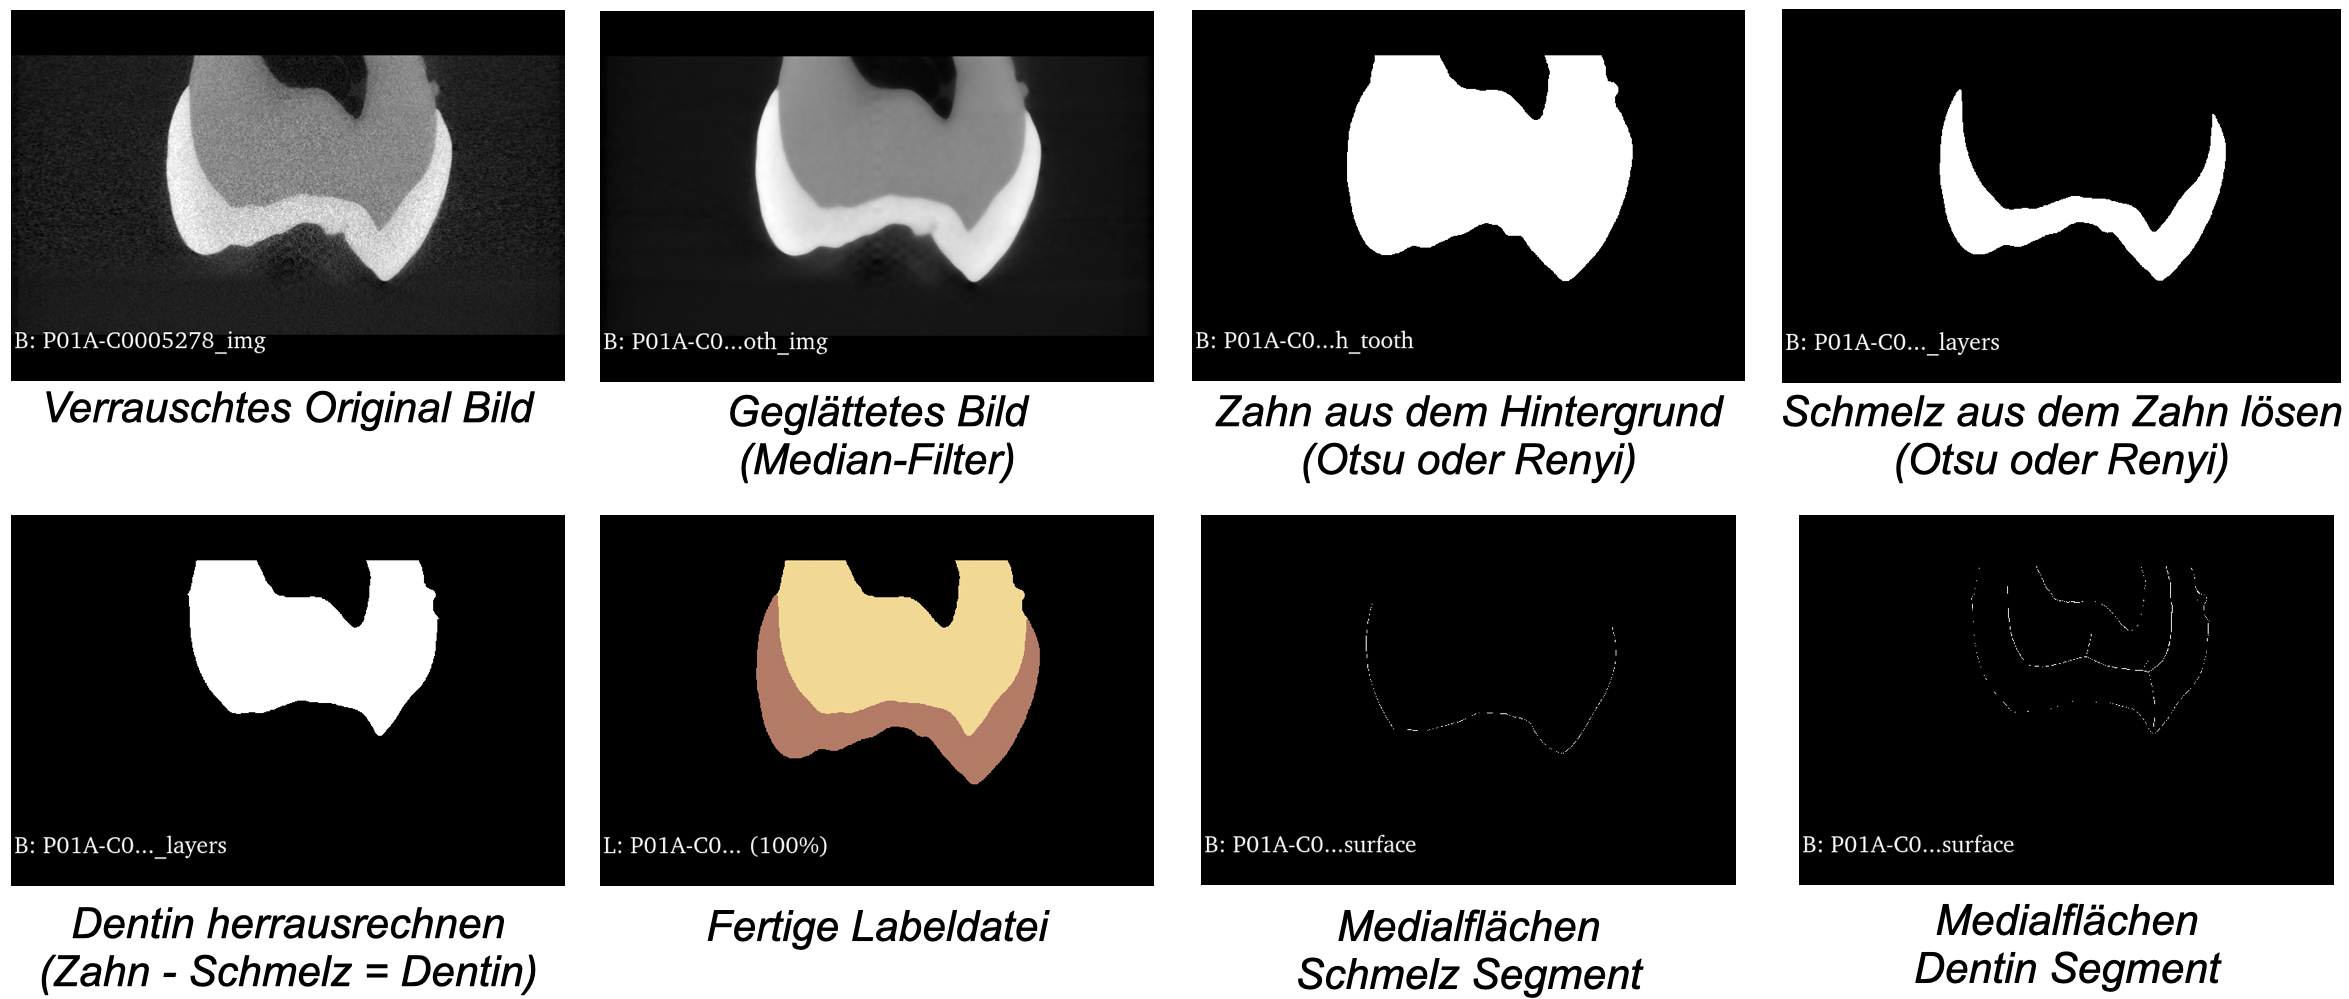
\includegraphics[width=0.8\textwidth]{img/anatomischeSegmentierung.png}
	\caption{Algorithmische formulierung der anatomischen Segmentierung nach
	\citet{hoffmann2020}}
	\label{fig:anatomische_segmentierung}
\end{figure}

\citet[S.~55]{hoffmann2020} beschreibt, dass dieses Verfahren bis zu einem
gewissen Fortschritt des Karies durchgeführt werden konnte, da der Algorithmus diesbezüglich
seine Grenzen hat. Außerdem ist das Verfahren für die ordinalen \ac{ISQ}-Bilder erstellt
worden, deren Daten im Format \ac{16Int} vorliegen. Für die spätere Darstellung
der Ergebnisse kann eine überlappende Ansicht in einer Visualisierungssoftware
verwendet werden. So ergibt sich die Situation, dass der Algorithmus ein gutes
Ergebnis liefert, jedoch nicht benutzerfreundlich zu bedienen ist. Für das
Starten und visualisieren des Verfahrens sind aufwendige Befehle über das
Terminal zu tippen \citep[vgl.][S.~53]{hoffmann2020}. Genau an dieser Stelle
soll die vorliegende Arbeit anknüpfen und das Verfahren der anatomischen
Segmentierung so interaktiv und benutzerfreundlich gestalten.

Für eine interaktive Verarbeitung von 3D Bilddaten bieten sich einige
Möglichkeiten. Die wohl beste Lösung liefert 3D Slicer. Warum die Wahl auf diese
Plattform fiel und welche Vorteile daraus entstehen wird im folgenden Abschnitt
\ref{sec:3d_slicer} erläutert.
% ---------------------------------------------------------------------------------------

\section{Interaktive Bildbearbeitung mit 3D Slicer}
\label{sec:3d_slicer} 3D Slicer ist eine Open-Source-Plattform, die speziell für
die Verarbeitung von Bilddaten im medizinischen Kontext eingesetzt wird. Dabei
wird sie von einer aktiven Community regelmäßig gewartet und weiterentwickelt
\citep[vgl.][]{slicer2024}, \citep[vgl.][S.~3]{fedorov2012slicer}. Für Slicer
gibt es offiziell keine Nutzungsbeschränkung. Jedoch sei auch gesagt, dass 3D
Slicer nicht für die klinische Nutzung zugelassen ist. \citet[S.~7]{fedorov2012slicer}
macht deutlich, das 3D Slicer ausschließlich für die Forschung gedacht ist. Um
einen ersten Überblick über die Komponenten von Slicer zu erlangen, soll die Abbildung
\ref{fig:3d_slicer_oekosystem} betrachtet werden.

\begin{figure}[h]
	\centering
	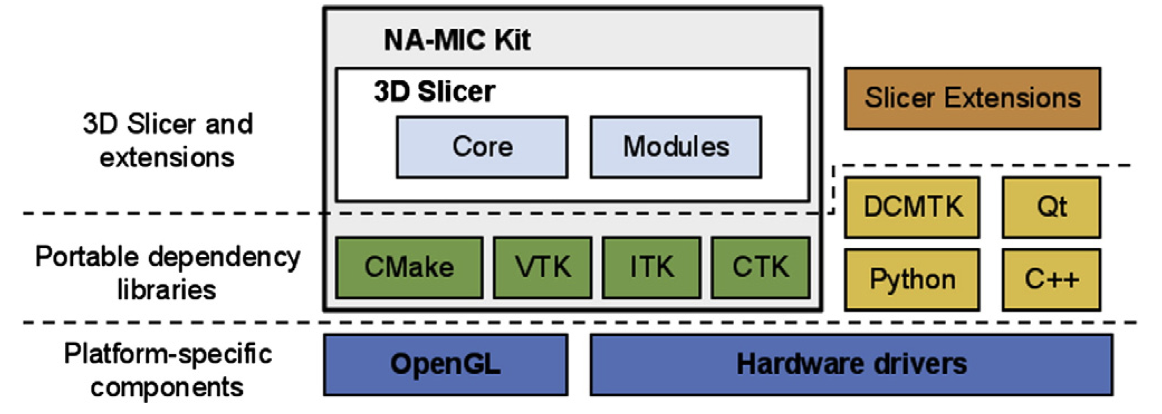
\includegraphics[width=0.9\textwidth]{img/3d_slicer_overview.jpg}
	\caption{3D Slicer Ökosystem nach \citet[S.~23]{fedorov2012slicer}}
	\label{fig:3d_slicer_oekosystem}
\end{figure}

\citet[S.~23]{fedorov2012slicer} teilt mit der Abbildung \ref{fig:3d_slicer_oekosystem}
die Plattform in drei Schichten auf. Auf der Obersten wird klar, dass 3D Slicer aus
der Kernanwendung und den installierbaren Modulen besteht. Neben den bereits
vorhandenen Modulen können von externen Entwicklern Module über die Slicer
Erweiterung entwickelt und bereitgestellt werden. Um eine Weiterentwicklung möglich
zu machen hat Slicer eine Reihe von Abhängigkeiten, die jedoch portabel gehalten
werden. Auf der untersten Schicht sind die Plattformspezifischen Anforderungen zu
sehen, die Slicer erfüllen soll.

So kommt es, dass das 3D Slicer Ökosystem sich durch einige Kriterien besonders auszeichnet.
Die wohl wichtigsten seien hier Stichpunktartig genannt \citep[vgl.][S.~11]{fedorov2012slicer}.

\begin{itemize}
	\item Kostenfreie Software

	\item Plug-in-Infrastruktur durch den \textit{Extension Manager}

	\item Ausführen von Skripten in der integrierten Python Konsole

	\item Verarbeitung von medizinischen Bilddaten von Kopf bis Fuß

	\item Interaktive Benutzerschnittstelle
\end{itemize}

3D Slicer hat für alle diese Punkte jeweils eine Lösung entwickelt, wobei der erste
Punkt durch die Open-Source-Philosophie schon gegeben ist. Die folgenden
Abschnitte decken diese Lösungen ab und bilden so eine erste Grundlage für die
Entwicklung mit 3D Slicer \citep[vgl.][S.~11]{fedorov2012slicer}.
% ---------------------------------------------------------------------------------------

\subsection{Extension Manager und Plug-in-Infrastruktur}
Der wohl bedeutendste Punkt ist die Plug-in-Infrastruktur, welche Slicer von
sich aus mitbringt. Um dieses Konzept genauer zu beleuchten, teilt man die
Plattform am besten in zwei Teile auf, die Kernanwendung und die Module, welcher
jeder Anwender personalisiert installieren oder deinstallieren kann. Diese Module
werden als \textit{Slicer lodabel module} bezeichnet \citep[vgl.][S.~25]{fedorov2012slicer}.
Slicer realisiert die Struktur durch den \textit{Extension Manager}, welcher
durchaus vergleichbar ist mit einer Art App-Store. Über diesen können bequem und
mit wenig Klicks die gewünschten Erweiterungen in das Kernsystem installiert werden.

\begin{minipage}{0.30\textwidth}
	Neben der Möglichkeit Module zu installieren bietet Slicer noch die Möglichkeit
	eigenen Module zu bauen und Sie im \textit{Extension Manager} zu
	veröffentlichen. Diese werden als \ac{SEM} bezeichnet. Hierzu verfolgt Slicer den
	Ansatz, dass jeder Entwickler eines Moduls selbst verantwortlich für Wartung
	und Weiterentwicklung ist, auch nachdem ein Paket veröffentlicht wurde \citep[vgl.][]{slicer2024}.
\end{minipage}
\hfill
\begin{minipage}{0.60\textwidth}
	\centering
	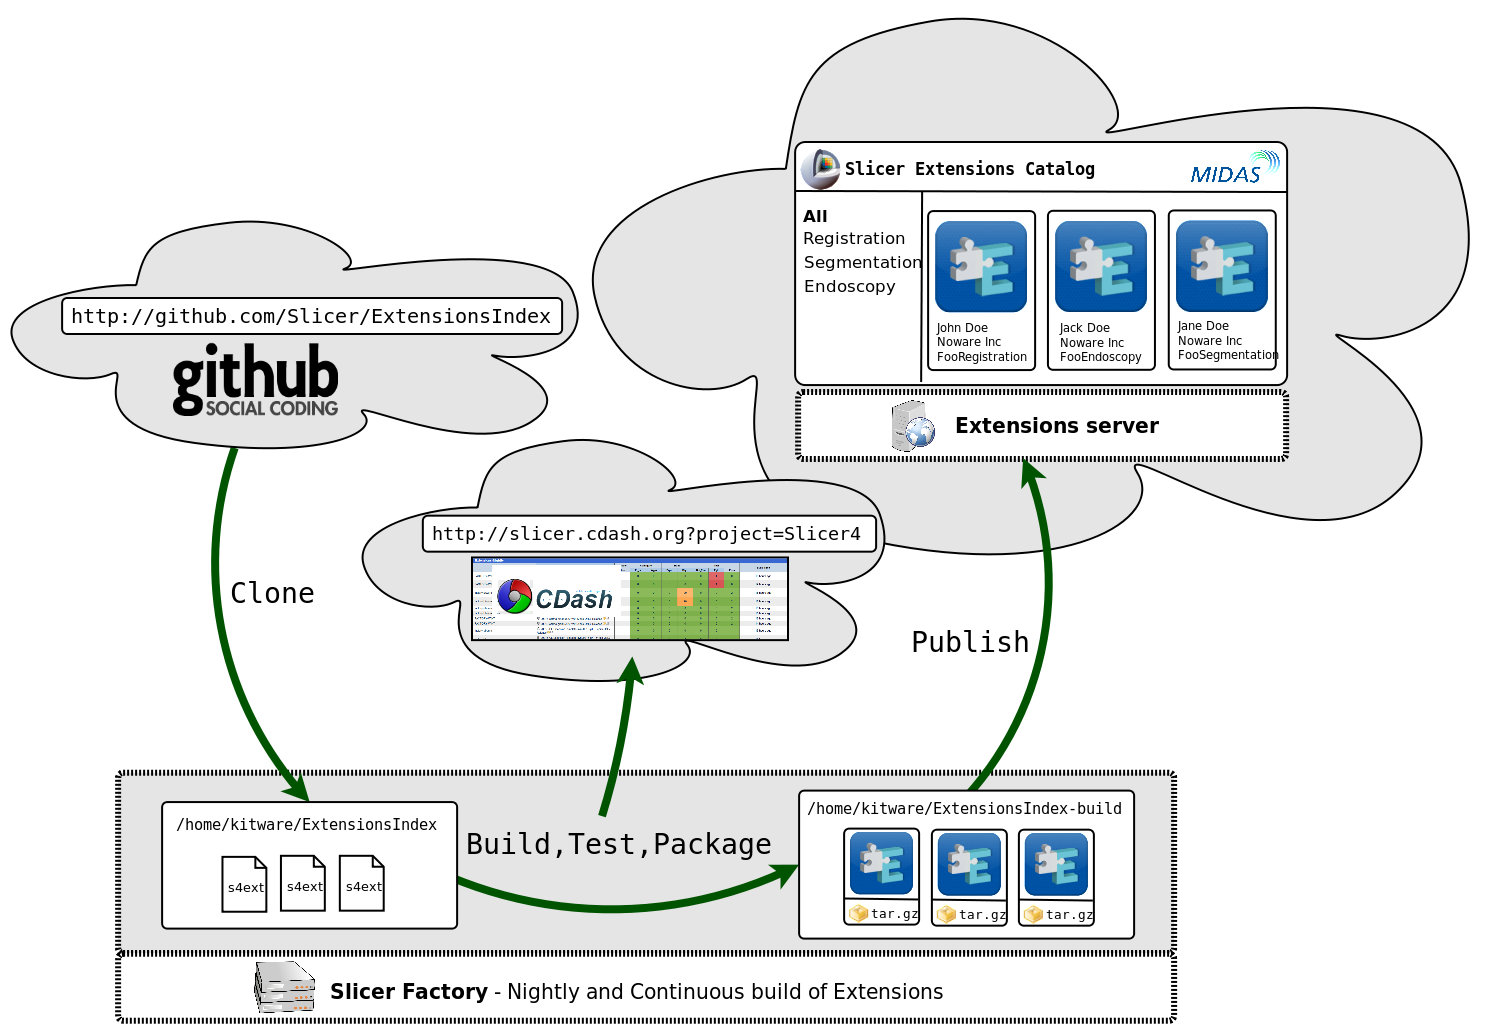
\includegraphics[width=1\textwidth]{img/slicer_extention_index.png}
	\captionof{figure}{Funktionsweise der Plug-in-Infrastruktur von 3D Slicer nach \citet{extensionsIndex2024}}
	\label{fig:3d_slicer_extension_index}
\end{minipage}

Slicer realisiert dies, indem die Plattform über ein zusätzliches Repository verfügt,
dass sich
\href{https://github.com/Slicer/ExtensionsIndex?tab=readme-ov-file}{\textit{ExtensionIndex}}
nennt. Dieses öffentliche Repository ist eine Auflistung aller \ac{SEM}. Die Auflistung
erfolgt durch eine Reihe an \ac{JSON} Dateien, die auf die Repositorien der einzelnen
Entwickler verweisen. Dieser
\href{https://github.com/Slicer/ExtensionsIndex?tab=readme-ov-file}{\textit{ExtensionIndex}}
ist über die Slicer Factory an den Extention Server und damit auch an den
Extention Manager angebunden. Die Slicer Factory ist ein System, das aus einem
Slicer Extention Repository ein lauffähiges Build erstellt, welches in den Extention
Katalog eingebunden werden kann. Ist eine Erweiterung in dem Erweiterungskatalog
gelistet, so sorgt der \textit{Extension Manager} dafür, dass die von der Slicer
Factory erstellt Build-Datei installiert werden kann. Abbildung
\ref{fig:3d_slicer_extension_index} soll diesen Vorgang verdeutlichen \citep[vgl.][]{slicer2024}.

Die Kernanwendung von 3D Slicer folgt einem Entwurfsmuster, dass sich \ac{MVC} nennt.
Bei der Erstellung einer \ac{SEM} soll dieser Ansatz ebenfalls gepflegt werden.
Eine High Level Betrachtung der Softwarearchitektur von 3D Slicer bietet
\cite[Seite 1332]{fedorov2012slicer} mit der Abbildung
\ref{fig:3d_slicer_architektur}.

\begin{figure}[h]
	\centering
	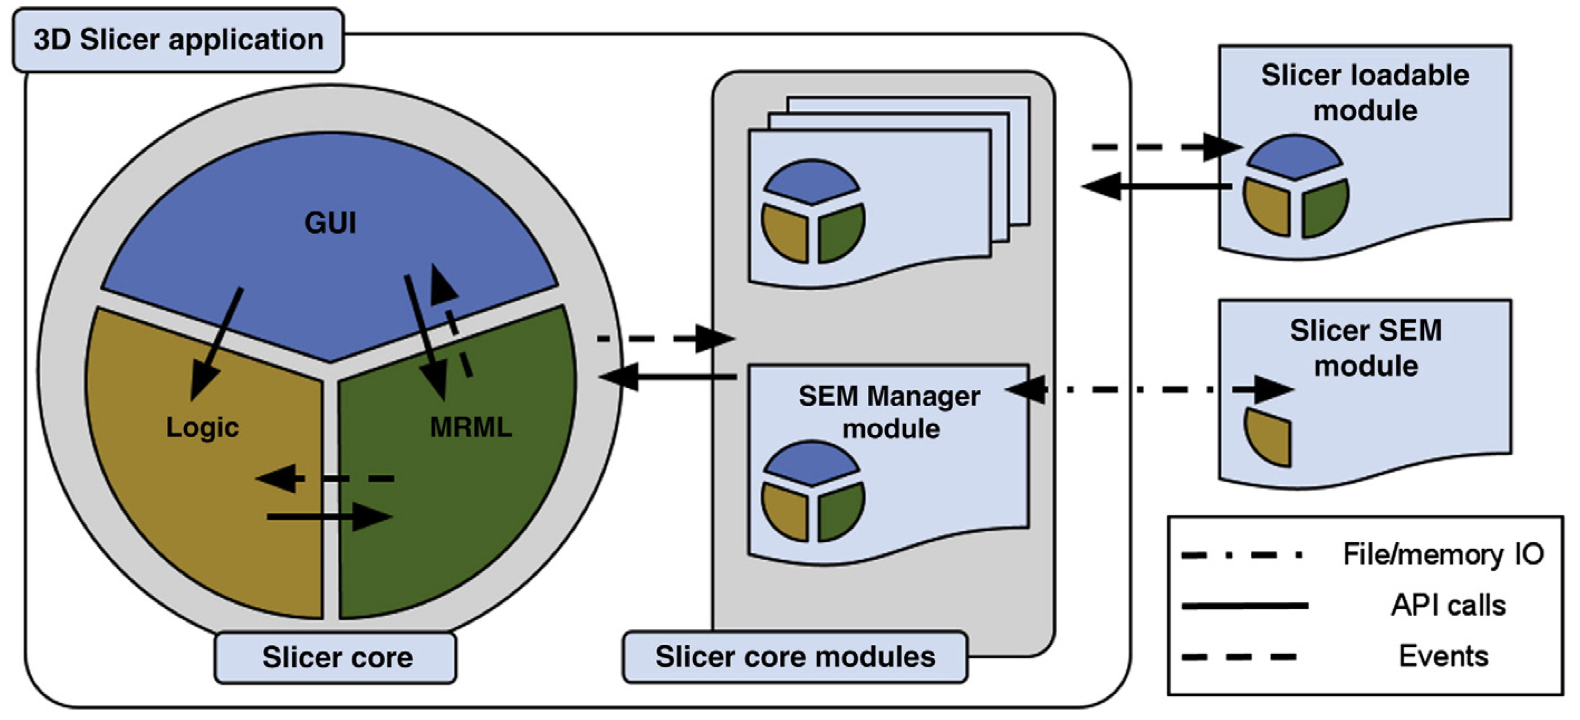
\includegraphics[width=0.9\textwidth]{img/3d_slicer_architektur.jpg}
	\caption{3D Slicer High Level Architektur nach \citet[S.~25]{fedorov2012slicer}}
	\label{fig:3d_slicer_architektur}
\end{figure}

Das Zusammenspiel zwischen \ac{MRML}, \ac{GUI} und der Logik bilden das MVC-Pattern
in der Kernanwendung. Das identische Pattern spiegelt sich auch in den einzelnen
Modulen von Slicer wieder. So wird sichergestellt, dass ein Softwareentwicklungsparadigma
eingehalten wird, was sich \textit{separation of concerns} nennt. Die Kapselung
von zusammengehöriger Logik. Bei der Erstellung einer eigenen Erweiterung ist die
Idee, dass nur die Logik implementiert werden muss und die komplexe Architektur
von Slicer erstmal nicht relevant ist.

Jedoch bietet sich in Slicer nicht nur die Möglichkeit eigene Erweiterungen zu
erstellen, es lässt sich hierfür auch die integrierte Python Konsole nutzen.
% ---------------------------------------------------------------------------------------

\subsection{Python Umgebung}
\label{subsec:pythob_umgebung} 3D Slicer bringt eine integrierte Python Konsole mit,
über die mit der Datenstruktur interagiert werden kann. So ist es möglich,
Python Skripte direkt in der Konsole auszuführen. Um dies zu realisieren, bringt
Slicer mit der Installation im jeweiligen Betriebssystem eine eigene Python
Umgebung mit. Dieses sieht wie folgt aus.

\begin{center}
	\texttt{./Slicer/bin/PythonSlicer}
\end{center}

Diese Python Umgebung verfügt über alle notwendigen Abhängigkeiten und Pakete. Bei
der Entwicklung eines \ac{SEM} kann dann auf das \ac{PyPi} in der integrierten Python
Umgebung zurückgegriffen werden. So kommt es, dass für eine Entwicklung mit Slicer
keine eigenen Python Umgebung auf der lokalen Maschine installiert sein muss.
Slicer bringt hier alles mit.

Für den letzten charakteristischen Punkt von Slicer aus Kapitel
\ref{sec:3d_slicer} führt der nächste Abschnitt in die durchaus komplexe
Datenstruktur \ac{MRML} ein, die bei einer Entwicklung mit Slicer unausweichlich
zu berücksichtigen ist.
% ---------------------------------------------------------------------------------------

\subsection{MRML Datenstruktur}
\label{subsec:mrml_datenstruktur} Die \ac{MRML}, gesprochen \textit{"Murlm"} ist
ein Datenmodell, das dafür entwickelt wurde, alle möglichen Bilddaten zu visualisieren
und zu speichern, die für einen klinischen Zweck Einsatz finden \citep[vgl.][]{slicer2024}.
Laut \citet{slicer2024} wurde die \ac{MRML}-Datenstruktur völlig unabhängig von
der Slicer Kernanwendung entwickelt. Dies ermöglicht ein Portieren der Datenstruktur
auf andere Softwareapplikationen. Da Slicer die einzig große Plattform ist, die diese
Datenstruktur nutzt, wird der Quellcode für \ac{MRML} im Repository von 3D Slicer
gewartet und weiterentwickelt, so \citet{slicer2024}. Durch den Artikel von
\citet[S.1]{fedorov2012slicer} wird klar, dass \ac{MRML} mehr ist also nur eine Datenstruktur.
Sie beschreiben \ac{MRML} als Szenenorganisator von Bilder, Annotationen, Layouts
und Anwendungsdaten.

\citet[S.~11]{fedorov2012slicer} beschreiben die \ac{MRML}-Datenstruktur als Schlüsselkomponenten
innerhalb von 3D Slicer. Dies ist auf die Softwarearchitektur von Slicer
zurückzuführen, die in Abbildung \ref{fig:3d_slicer_architektur} beschrieben wurde.
Die Kernanwendung von Slicer arbeitet wie bereits beschrieben nach dem \ac{MVC}-Pattern.
\ac{MRML} übernimmt hier den Teil des \textit{Models (M)} und bildet damit den
Grundstein der Anwendung \citep[vgl.][S.~25]{fedorov2012slicer}.

\citet{slicer2024} und der Artikel von \citet[S.~11]{fedorov2012slicer} beschreibt
\ac{MRML} als \ac{XML}-Format. Wird also eine \ac{MRML}-Szene gespeichert, so
folgt eine Speicherung als \ac{MRML}-Datei und damit unter der Haube als \ac{XML}-Datei.
Dabei wird laut \citet{slicer2024} nur eine Referenz auf das Bild gespeichert. Die
zu bearbeitende Aufnahme selbst wird nicht innerhalb einer \ac{MRML}-Datei
abgespeichert.

\ac{MRML} zeichnet sich vor allem dadurch aus, dass es eine Vielzahl an
Dateiformaten akzeptiert. Alle Formate, die für einen klinischen Zweck
verarbeitet werden, können durch \ac{MRML} unterstützt werden. Um dies zu gewährleisten,
ist die \ac{MRML}-Szene in sogenannte Knoten (engl.: nodes) aufgeteilt. Die
Basistypen für einen Knoten folgen der \citet{slicer2024} und sind in der folgenden
Aufzählung zu sehen.

\begin{minipage}{0.45\textwidth}
	\begin{itemize}
		\item Data node

		\item Display node

		\item Storage node

		\item View node
	\end{itemize}
\end{minipage}
\hfill
\begin{minipage}{0.45\textwidth}
	\begin{itemize}
		\item Plot node

		\item Subject hierarchy node

		\item Sequence node

		\item Parameter node
	\end{itemize}
\end{minipage}

Wird also ein Bild in eine \ac{MRML}-Szene geladen, so speichert Slicer die
unterschiedlichen Eigenschaften eines Bildes in unterschiedlichen Knoten. So werden
Beispielsweise Basiseigenschaften einer Probe im \textit{Data node} gespeichert,
wo hingegen ein \textit{Storage node} beschreibt wie ein Bild auf der Festplatte
gespeichert wird. In \textit{Display node} werden die Eigenschaften zur
Darstellung eines Bildes hinterlegt. Der Hintergrund für die Speicherung von Probendaten
in unterschiedlichen Knoten ist, dass beispielsweise dasselbe Bild in
unterschiedlichen Formaten vorliegt oder ein und dasselbe Bild auf zwei
unterschiedliche Arten visualisiert werden soll. So kann sich beispielsweise eine
Struktur wie in Abbildung \ref{fig:3d_slicer_class} ergeben.

\begin{figure}[h]
	\centering
	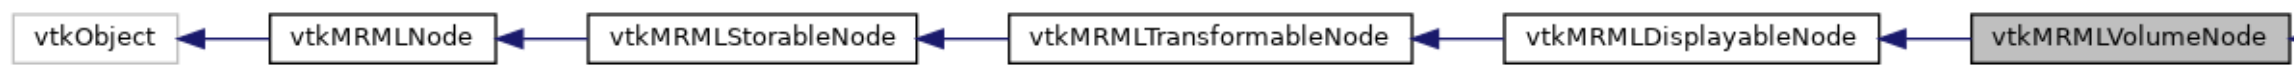
\includegraphics[width=1\textwidth]{img/slicer_class_index.jpg}
	\caption{3D Slicer High Level Architektur nach \citet{slicer2024}}
	\label{fig:3d_slicer_class}
\end{figure}

Die Informationen in einem Bild werden also über diese Typen aufgeteilt und je
nach Sinn abgespeichert. Möchte man demnach auf die bestimmte Informationen in einer
Probe zugreifen. So kann diese Information über den Aufruf bestimmter Methoden
erfolgen

\begin{lstlisting}[
	language={python},
	caption={Auslesen der Informationen aus den verschiedenen Knoten},
	label={lst:_auslehsen_nodes}]
# data node - vtkMRMLVolumeNode
currentVolume.GetImageData()
# storage node - vtkMRMLStorableNode
currentVolume.GetStorageNode()
# display node - vtkMRMLDisplayableNode
currentVolume.GetDisplayNode()
\end{lstlisting}

Wie die Kommentare in Listing \ref{lst:_auslehsen_nodes} bereits zeigen, gibt es
noch eine Besonderheit von \ac{MRML}. Damit eine Verwaltung aller Dateiformate möglich
ist, bedient sich \ac{MRML} einiger Tools, die sich bereits etabliert haben. Die
Wichtigsten sind hierbei \ac{VTK} und \ac{ITK} \citep[vgl.][K.~1.1]{vtk2006}, \citep[vgl.][K.~1.1]{itkguide2015}.
Die beiden Tools sind echte Riesen in ihrer Branche. \ac{MRML} nutzt diese, um
einige Dateiformate zu lesen und zu schreiben.

Durch das Betrachten der \ac{MRML}-Szene wird klar, dass Slicer hierdurch viele
Möglichkeiten bietet. Speziell für die effiziente Speicherung der Proben in einer
Szene durch die unterschiedlichen Knotentypen. Ein besonderer Knoten, der gleichzeitig
auch die Brücke zu der interaktiven Benutzerschnittstelle von Slicer baut, ist
der \textit{Parameter node}. Warum dieser eine zentrale Rolle spielt und wie
Slicer die Schnittstelle grundsätzlich gestaltet, soll in Kapitel \ref{subsec:benutzerschnitstelle}
Benutzerschnittstelle diskutiert werden.
% ---------------------------------------------------------------------------------------

\subsection{Benutzerschnittstelle}
\label{subsec:benutzerschnitstelle} Für das Erstellen einer \ac{UI}, die für eine
Slicer Erweiterung notwendig ist, nutzt 3D Slicer den Qt-Designer \citep[vgl.][Ab.~Einführung]{qt2024}.
Die Integration des Qt-Designers als Applikation in eine andere Applikation
funktioniert aufgrund der Plattformintegrität, die der Designer mitbringt \citep[vgl.][Ab.~Einführung]{qt2024}.
Diese bietet so die Möglichkeit die benötigten Widgets über eine interaktive Benutzerschnittstelle
zu bauen. Für diese \ac{UI}-Vorrichtung gibt es einen Gegenspieler im Quelltext des
Programmes, welcher als \textit{ParameterNode} bekannt ist. Der \textit{ParameterNode}
ist laut \citet{slicer2024} eine leichte Variante eines \ac{MRML}-Knoten um Parametereinstellungen
zu speichern. Durch das Zusammenspiel zwischen \ac{UI} und \textit{ParameterNode}
wird die \ac{UI} automatisch aktualisiert, wenn sich das Programm ändert und
umgekehrt, so erklärt es die \citet{slicer2024}.

\begin{minipage}{0.35\textwidth}
	Das Erstellen der Verknüpfung zwischen \ac{UI}-Widget und \textit{ParameterNode}
	erfolgt über die dynamische Eigenschaft \texttt{SlicerParameterName}, die direkt
	in der Bombenentenansicht im Qt-Designer einstellbar ist. Die Abbildung
	\ref{fig:qt_designer} soll diesen Vorgang verdeutlichen. Diese Verknüpfung lässt
	sich laut \citet{slicer2024} auch via Programmcode setzten.
\end{minipage}
\hfill
\begin{minipage}{0.55\textwidth}
	\centering
	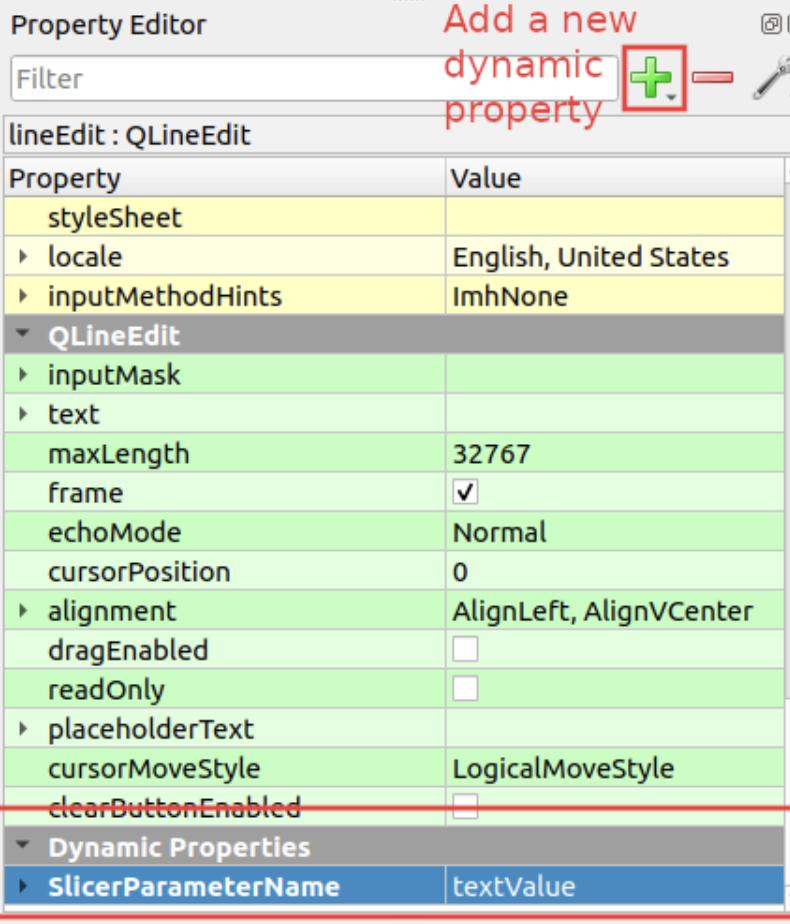
\includegraphics[width=0.5\textwidth]{img/qt_designer.jpg}
	\captionof{figure}{Dynamische Eigenschaft einer Komponente im Qt-Designer nach der \citet{slicer2024}}
	\label{fig:qt_designer}
\end{minipage}

\begin{center}
	\texttt{widget.setProperty('SlicerParameterName', 'parameterName')}
\end{center}

Über das Objekt \texttt{widget} kann die Eigenschaft einer Komponente gesetzt werden,
ohne dass sie im Designer berührt werden muss.

Mit dem Ende dieses Abschnittes wurden alle wichtigen Bestandteile von 3D Slicer
abgedeckt und diskutiert, sowie alle weiteren Domänen eingeführt. So bleibt nun
die Frage nach dem Sinn dieser Arbeit. Das Kapitel \ref{chap:fragestellung} soll
hier Klarheit liefern und die konkrete Fragestellung ausarbeiten.
% ---------------------------------------------------------------------------------------